% Name: Rotation about a point
% Description: Triangle ABC turned 90° counterclockwise about the origin to A′B′C′: OC and OC′ are equal and at right angles, and C moves along the arc between them.
% Tags: transformation, rotation, center of rotation, coordinate geometry

\usetikzlibrary{arrows.meta, angles}

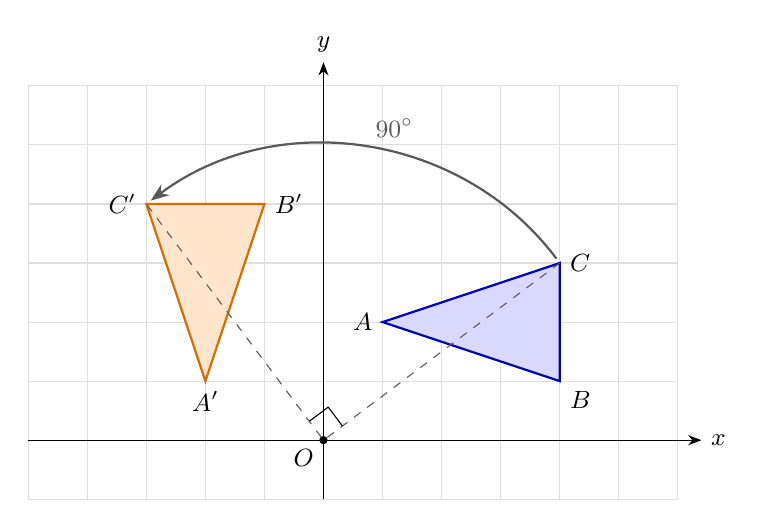
\begin{tikzpicture}[>={Stealth}, scale=0.75, every node/.style={font=\small}]
  % (x, y) maps to (-y, x); C = (4, 3) is 5 from O, at 36.87 degrees
  \draw[gray!25] (-5,-1) grid (6,6);
  \draw[->] (-5,0) -- (6.4,0) node[right] {$x$};
  \draw[->] (0,-1) -- (0,6.4) node[above] {$y$};
  \coordinate (O) at (0,0);
  \coordinate (C) at (4,3);
  \coordinate (C') at (-3,4);
  \draw[->, thick, gray!70!black, shorten >=2pt, shorten <=2pt] (C) arc[start angle=36.87, end angle=126.87, radius=5] node[pos=0.5, above right] {$90^\circ$};
  \draw[thick, fill=blue!15, draw=blue!70!black] (1,2) node[left] {$A$} -- (4,1) node[below right] {$B$} -- (C) node[right] {$C$} -- cycle;
  \draw[thick, fill=orange!20, draw=orange!85!black] (-2,1) node[below] {$A'$} -- (-1,4) node[right] {$B'$} -- (C') node[left] {$C'$} -- cycle;
  \draw[dashed, gray!70!black] (C) -- (O) -- (C');
  \pic[draw, angle radius=3mm] {right angle=C--O--C'};
  \fill (O) circle (2pt) node[below left] {$O$};
\end{tikzpicture}
